%%%%%%%%%%%%%%%%%%%%%%%%%%%%%%%%%%%%%%%%%
% baposter Landscape Poster
% LaTeX Template
% Version 1.0 (11/06/13)
%
% baposter Class Created by:
% Brian Amberg (baposter@brian-amberg.de)
%
% This template has been downloaded from:
% http://www.LaTeXTemplates.com
%
% License:
% CC BY-NC-SA 3.0 (http://creativecommons.org/licenses/by-nc-sa/3.0/)
%
%%%%%%%%%%%%%%%%%%%%%%%%%%%%%%%%%%%%%%%%%

%----------------------------------------------------------------------------------------
%	PACKAGES AND OTHER DOCUMENT CONFIGURATIONS
%----------------------------------------------------------------------------------------

\documentclass[landscape,a0paper,fontscale=0.3]{baposter} % Adjust the font scale/size here

\usepackage{graphicx} % Required for including images
\graphicspath{{figures/}} % Directory in which figures are stored

\usepackage[utf8]{inputenc}
\usepackage[T1]{fontenc}
\usepackage[french]{babel}
\usepackage{amsmath} % For typesetting math
\usepackage{amssymb} % Adds new symbols to be used in math mode

\usepackage{booktabs} % Top and bottom rules for tables
\usepackage{enumitem} % Used to reduce itemize/enumerate spacing
\usepackage{palatino} % Use the Palatino font
\usepackage[font=small,labelfont=bf]{caption} % Required for specifying captions to tables and figures

\usepackage{multicol} 
\usepackage{float} % Required for multiple columns
\usepackage{placeins} 
\usepackage{stfloats} 

\setlength{\columnsep}{1.5em} % Slightly increase the space between columns
\setlength{\columnseprule}{0mm} % No horizontal rule between columns
\selectcolormodel{cmyk}

\usepackage{tikz} % Required for flow chart
\usetikzlibrary{shapes,arrows} % Tikz libraries required for the flow chart in the template

\newcommand{\compresslist}{ % Define a command to reduce spacing within itemize/enumerate environments, this is used right after \begin{itemize} or \begin{enumerate}
\setlength{\itemsep}{1pt}
\setlength{\parskip}{0pt}
\setlength{\parsep}{0pt}
}

\definecolor{darkgreen}{cmyk}{0.2394,0.0000,0.2394,0.2627}
\definecolor{orange}{cmyk}{0.0000,0.7294,1.0000,0.0000} 
\definecolor{floralwhite}{cmyk}{0.0000,0.0196,0.0588,0.0000}
\definecolor{gray}{cmyk}{0.0000,0.0000,0.0000,0.0392}
\definecolor{lightgreen}{cmyk}{0.7554,0.0000,0.7554,0.4549}
\definecolor{lightblue}{rgb}{0.145,0.6666,1} % Defines the color used for content box headers

\begin{document}

\begin{poster}
{
headerborder=closed, % Adds a border around the header of content boxes
colspacing=1em, % Column spacing
bgColorOne=floralwhite, % Background color for the gradient on the left side of the poster
bgColorTwo=white, % Background color for the gradient on the right side of the poster
borderColor=lightgreen, % Border color
headerColorOne=lightgreen, % Background color for the header in the content boxes (left side)
headerColorTwo=white, % Background color for the header in the content boxes (right side)
headerFontColor=white, % Text color for the header text in the content boxes
boxColorOne=white, % Background color of the content boxes
textborder=roundedleft, % Format of the border around content boxes, can be: none, bars, coils, triangles, rectangle, rounded, roundedsmall, roundedright or faded
eyecatcher=true, % Set to false for ignoring the left logo in the title and move the title left
headerheight=0.1\textheight, % Height of the header
headershape=roundedright, % Specify the rounded corner in the content box headers, can be: rectangle, small-rounded, roundedright, roundedleft or rounded
headerfont=\large\bf\textsc, % Large, bold and sans serif font in the headers of content boxes
%textfont={\setlength{\parindent}{1.5em}}, % Uncomment for paragraph indentation
linewidth=2pt % Width of the border lines around content boxes
}
%----------------------------------------------------------------------------------------
%	TITLE SECTION 
%----------------------------------------------------------------------------------------
%
{
\includegraphics[height=6em]{logo_lip_HD}} % First university/lab logo on the left
{\bf\Large\textcolor{orange}{Caractérisation et Méthodologie d'Analyse des Buffer Overflow }\vspace{0.2em}} % Poster title
{\textsl{ \small Yves KONE, Alain TCHANA \{Ecole Normale Supérieure de Lyon\}\\ \vspace{0.2em}

\includegraphics[width=0.2\linewidth]{compas18}}} % Author names and institution
{
\includegraphics[height=6em]{enslogo}} % Second university/lab logo on the right

%----------------------------------------------------------------------------------------
%	OBJECTIVES
%----------------------------------------------------------------------------------------

\headerbox{Common Vulnerabilities and Exposures}{name=cve,column=0,row=0,span=2}{
Les CVE pour Common Vuln\'erabilites and Exposures est une base de donn\'ees publique r\'epertoriant des vuln\'erabili\'es de s\'ecurit\'e.
Chaque CVE est compos\'e de 2 parties disctinctes:
\begin{itemize}
	\item le descriptif principal qui pr\'esente bri\`evement la vuln\'erabilit\'e.
    \item les r\'ef\'erences qui sont des URLs vers des pages web de diff\'erents types.
\end{itemize}
\begin{center}
    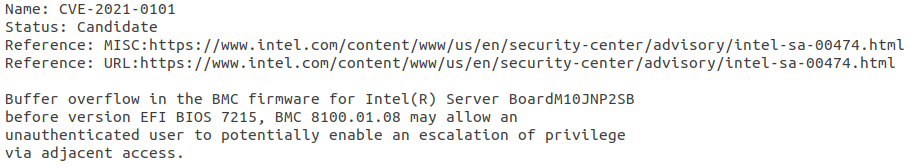
\includegraphics[width=\linewidth]{cve_entry}
    \captionof{figure}{Exemple d'un CVE concernant les buffer overflow en 2021.}
    \end{center}
%\vspace{0.1em} % When there are two boxes, some whitespace may need to be added if the one on the right has more content
}

\headerbox{Catégorisation}{name=categorie,column=1, below=cve, span=1}{
Cat\'etgorisation et extraction et interpr\'etation des informations
Notre objectif est de proposer une m\'ethodologie d'analyse des CVEs de type BOF et concevoir un outil d'analyse automatique.
Nous avions donc un besoin d'identifier les caract\'eristiques des BOF:
Apr\`es plusieurs passages, nous avons cat\'egories suivantes:
\begin{itemize}
    \item \bf le type de d\'ebordement;
    \item \bf la zone m\'emoire;
    \item \bf les cons\'equences ou effets;
    \item \bf le contexte relatif au code;
    \item \bf le syst\`eme impact\'e;
    \item \bf la compagnie, entreprise impact\'ee.
\end{itemize}
}
%----------------------------------------------------------------------------------------
%	RESULTS 
%----------------------------------------------------------------------------------------

\headerbox{Méthodologie}{name=contrib,column=2,span=2,row=0, aligned=cve, bottomaligned=categorie}{
    L'algorithme consiste \`a analyser le descriptif principal puis les r\'ef\'erences.
    Pour analyser le descriptif il faut extraire les informations pertinente et les interpréter.
    \newline
    \newline
    Pour les références c'est un peu plus subtil. Il faut d'abord, en fonction du type de page web, 
    identifier les sources d'information puis extraire celles qui nous intéressent et ensuite les interpréter
    \begin{figure}[H]
        \centering
        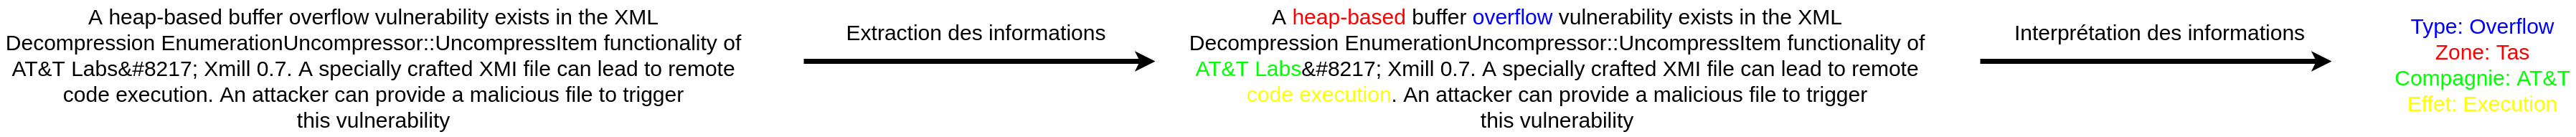
\includegraphics[width=17cm, height=1cm]{descriptif}
        \captionof{figure}{Automate simplifié de l'analyse d'un CVE.}
    \end{figure}
    L'algorithme consiste à analyser le descriptif principal puis les références.
    Pour analyser le descriptif il faut extraire les informations pertinente et les interpréter.\\
    \begin{figure}[H]
        \centering
        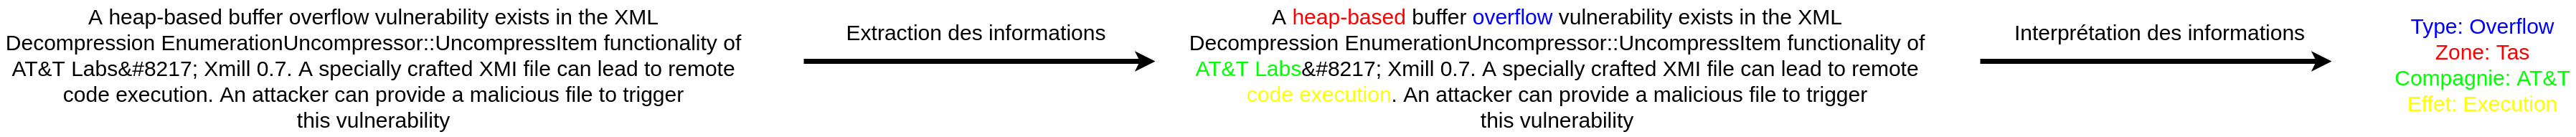
\includegraphics[width=17cm, height=1cm]{descriptif}
        \captionof{figure}{Automate simplifié de l'analyse d'un CVE.}
    \end{figure}
}

%----------------------------------------------------------------------------------------
%	REFERENCES
%----------------------------------------------------------------------------------------



%----------------------------------------------------------------------------------------
%	CONTACT INFORMATION
%----------------------------------------------------------------------------------------


%----------------------------------------------------------------------------------------
%	CONTRIB
%----------------------------------------------------------------------------------------



%----------------------------------------------------------------------------------------
%	PROBLEM
%----------------------------------------------------------------------------------------





\headerbox{Problematique}{name=problem,column=0,below=cve, bottomaligned=categorie}{ % This block's bottom aligns with the bottom of the conclusion block
Les CVEs constituent un Dataset important pour la recherche en s\'ecurit\'e (\textcolor{orange}{12669} CVE concernant les overflow depuis 2013).
Neanmoins, une analyse fine et pertinente des CVEs peut s'av\'erer etre une tache tr\`es longue et fastidieuse.\newline
A titre d'exemple nous avons pass\'e plus de 6 mois (et plusieurs bo\^ites de vitamines) pour obtenir nos premiers r\'esultats.
Les principales cause sont:
\begin{itemize}
    \item \bf\textcolor{orange}{le grand nombre de CVE r\'epertori\'e;}
	\item \bf\textcolor{orange}{les donn\'ees sont non structur\'ees, parser les CVE ne suffit pas;} 
    \item \bf\textcolor{orange}{pas de m\'ethode d'analyse ou d'outil automatique, il faut tout faire a la main.}
\end{itemize}
}





\headerbox{Resultats pr\'eliminaires}{name=results,column=2,span=2,row=1,below=contrib, boxColorOne=floralwhite}{
Nous avons obtenus quelques résultats
\begin{multicols*}{2}
\end{multicols*}
}
%----------------------------------------------------------------------------------------
%	MOTIV
%----------------------------------------------------------------------------------------

%----------------------------------------------------------------------------------------
\headerbox{References}{name=references,column=0,below=problem, span=2,boxColorOne=floralwhite}{

\renewcommand{\section}[2]{\vskip 0.05em} % Get rid of the default "References" section title
\nocite{*} % Insert publications even if they are not cited in the poster
\small{ % Reduce the font size in this block
\bibliographystyle{unsrt}
\bibliography{sample} % Use sample.bib as the bibliography file
}}


\headerbox{Contact}{name=contact,column=0,below=references,boxColorOne=floralwhite}{ % This block is as tall as the references block

\begin{description}\compresslist
\item[Linkedin] 
\item[Email] yves.kone@ens-lyon.fr
\end{description}
}
\end{poster}

\end{document}